\documentclass[aspectratio=169, lualatex, handout]{beamer}
\makeatletter\def\input@path{{theme/}}\makeatother\usetheme{cipher}

\title{Applied Cryptography}
\author{Nadim Kobeissi}
\institute{American University of Beirut}
\instituteimage{images/aub_white.png}
\date{\today}
\coversubtitle{CMPS 297AD/396AI\\Fall 2025}
\coverpartname{Part 1: Provable Security}
\covertopicname{1.2: One-Time Pad \& The Provable Security Mindset}
\coverwebsite{https://appliedcryptography.page}

\begin{document}
\begin{frame}[plain]
	\titlepage
\end{frame}

\begin{frame}{How it's made}
	\bigimagewithcaption{fischer_theory.png}{Fischer et al., The Challenges of Bringing Cryptography from Research Papers to Products: Results from an Interview Study with Experts, USENIX Security 2024}
\end{frame}

\begin{frame}{Thinking about secrecy}
	\bigimagewithcaption{naive_enc.pdf}{Source: The Joy of Cryptography}
\end{frame}

\begin{frame}{Thinking about secrecy}
	\begin{columns}[c]
		\column{0.5\textwidth}{
			\begin{itemize}[<+->]
				\item Keep the whole design secret?
				\item \textbf{``Advantages''}:
				      \begin{itemize}[<+->]
					      \item Attacker doesn't know how our cipher (or system, more generally,) works.
				      \end{itemize}
				\item \textbf{Disadvantages}:
				      \begin{itemize}[<+->]
					      \item Figuring out how the thing works might mean a break.
					      \item Can't expose cipher to scrutiny.
					      \item Everyone needs to invent a cipher.
				      \end{itemize}
			\end{itemize}
		}
		\column{0.5\textwidth}{
			\imagewithcaption{naive_enc.pdf}{Source: The Joy of Cryptography}
		}
	\end{columns}
\end{frame}

\begin{frame}{Kerckhoff's principle}
	\begin{itemize}[<+->]
		\item \textit{``A cryptosystem should be secure even if everything about the system, except the key, is public knowledge.''} — Auguste Kerckhoffs, 1883
		\item \textbf{Why it matters}:
		      \begin{itemize}[<+->]
			      \item No ``security through obscurity''
			      \item The key is the only secret: the rest can be audited, tested, trusted
			      \item Encourages open standards and peer review
			      \item If your system's security depends on nobody knowing how it works, it's not secure.
		      \end{itemize}
	\end{itemize}
\end{frame}

\begin{frame}{Thinking about secrecy}
	\bigimagewithcaption{keyed_enc.pdf}{\textbf{Concentrate all the need for secrecy in the key!}}
\end{frame}

\begin{frame}{Thinking about secrecy}
	\begin{columns}[c]
		\column{0.5\textwidth}{
			\begin{itemize}[<+->]
				\item Cipher can be scrutinized, used by anyone.
				\item Design can be shown to hold so long as the key is secret.
				\item This is how virtually all cryptography is designed today.
			\end{itemize}
		}
		\column{0.5\textwidth}{
			\imagewithcaption{keyed_enc.pdf}{Source: The Joy of Cryptography}
		}
	\end{columns}
\end{frame}

\begin{frame}{One-time pad}{First look at a symmetric cipher}
	\begin{columns}[c]
		\begin{column}{0.5\textwidth}
			\sssubroutine{Enc}{K, M}{
				$C \coloneq K \oplus M$ \\
				return $C$
			}{2}
		\end{column}
		\begin{column}{0.5\textwidth}
			\sssubroutine{Dec}{K, C}{
				$M \coloneq K \oplus C$ \\
				return $M$
			}{2}
		\end{column}
	\end{columns}
\end{frame}

\begin{frame}{XOR (Exclusive OR) operation}
	\begin{columns}[c]
		\column{0.6\textwidth}{
			\begin{table}
				\centering
				\begin{tabular}{|c|c|c|}
					\hline
					\textbf{A} & \textbf{B} & \textbf{A $\oplus$ B} \\
					\hline
					\bit{0} & \bit{0} & \bit{0}            \\
					\hline
					\bit{0} & \bit{1} & \bit{1}            \\
					\hline
					\bit{1} & \bit{0} & \bit{1}            \\
					\hline
					\bit{1} & \bit{1} & \bit{0}            \\
					\hline
				\end{tabular}
				\caption{Truth table for XOR operation}
			\end{table}
			\begin{itemize}
				\item XOR returns 1 when inputs differ
				\item XOR returns 0 when inputs are the same
				\item Key property: $x \oplus x = 0$ and $x \oplus 0 = x$
				\item Self-inverse: $(M \oplus K) \oplus K = M$
			\end{itemize}
		}
		\column{0.4\textwidth}{
			\begin{center}
				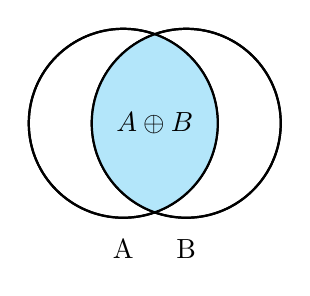
\begin{tikzpicture}[scale=0.8]
					\draw[thick] (0,0) circle (1.5);
					\draw[thick] (1,0) circle (1.5);
					\node at (0,-2) {A};
					\node at (1,-2) {B};
					\begin{scope}
						\clip (0,0) circle (1.5);
						\clip (1,0) circle (1.5);
						\fill[cyan!30] (-1.5,-1.5) rectangle (2.5,1.5);
					\end{scope}
					\draw[thick] (0,0) circle (1.5);
					\draw[thick] (1,0) circle (1.5);
					\node at (0.5,0) {$A \oplus B$};
				\end{tikzpicture}
			\end{center}
		}
	\end{columns}
\end{frame}

\begin{frame}{One-time pad}{First look at a symmetric cipher}
	\bigimagewithcaption{xor_enc.png}{(We're encoding the message and key as bits)}
\end{frame}

\begin{frame}{One-time pad}{First look at a symmetric cipher}
	\bigimagewithcaption{xor_dec.png}{(We're encoding the message and key as bits)}
\end{frame}

\begin{frame}{Key derivation}{Uniform distribution}
	\begin{itemize}[<+->]
		\item How to derive $K$?
		\item $K$ is ideally random.
		\item True randomness isn't practical, so $K$ is in practice pseudo-random.
		\item We need a pseudo-random uniform distribution:
		\item If $\mathcal{S}$ is a set of $m$ items, then the uniform distribution over $\mathcal{S}$ assigns probability $\frac{1}{m}$ to each item $x \in \mathcal{S}$
		\item In practice, this just means we need the bits to be random, unpredictable, uniformly distributed in terms of probability
		\item Sampling a $K$ from a pseudo-random uniform distribution is written as $K \twoheadleftarrow \bits^n$
	\end{itemize}
\end{frame}

\begin{frame}{Adversary's access to oracle}
	\begin{columns}[c]
		\begin{column}{0.5\textwidth}
			\begin{itemize}[<+->]
				\item ``Victim'' chooses their key.
				\item Adversary chooses the message and receives the ciphertext.
				\item We say that \textbf{the adversary has access to an encryption oracle}.
			\end{itemize}
		\end{column}
		\begin{column}{0.5\textwidth}
			\imagewithcaption{attacker_interface.pdf}{Source: The Joy of Cryptography}
		\end{column}
	\end{columns}
\end{frame}

\begin{frame}{Adversary's access to oracle}
	\begin{center}
		\begin{tikzpicture}[
				box/.style={rectangle, draw, minimum height=2.5cm, align=left, fill=white},
				dashed box/.style={rectangle, draw, dashed, minimum width=2.5cm, minimum height=2.5cm, align=center, fill=white},
				>=Stealth,
			]
			\node[dashed box] (adversary) {$adversary$};
			\node[box, right=2cm of adversary](attack){
				$\underline{\func{attack}{M}}$: \hfill \quad \quad \textcolor{gray}{\scriptsize \textit{// adversary chooses $M$}} \\
				\quad $K \twoheadleftarrow \bits^{n}$ \hfill \quad \quad \textcolor{gray}{\scriptsize \textit{// victim samples $K$}} \\
				\quad $C \coloneq \textsf{Enc}(K, M)$ \hfill \quad \quad \textcolor{gray}{\scriptsize \textit{// victim encrypts}} \\
				\quad return $C$ \hfill \quad \quad \textcolor{gray}{\scriptsize \textit{// adversary sees $C$}}
			};
			\draw[->] (adversary) -- node[above] {$M$} (attack);
			\draw[<-] ([yshift=-0.5cm]adversary.east) -- node[below] {$C$} ([yshift=-0.5cm]attack.west);
		\end{tikzpicture}
	\end{center}
\end{frame}

\begin{frame}{Adversary's access to oracle}
	\begin{columns}[c]
		\begin{column}{0.5\textwidth}
			\begin{itemize}[<+->]
				\item Adversary can query oracle an unbounded number of times.
				\item Two queries with same $M$ may return different $(C, C')$, since victim may use different $K$.
				\item $K$ is always chosen correctly (pseudo-random uniform sampling)
				\item ``Randomized oracle''
				\item Attacker cannot see $K$.
			\end{itemize}
		\end{column}
		\begin{column}{0.5\textwidth}
			\imagewithcaption{attacker_interface.pdf}{Source: The Joy of Cryptography}
		\end{column}
	\end{columns}
\end{frame}

\begin{frame}{Adversary's access to oracle}
	\begin{columns}[c]
		\begin{column}{0.5\textwidth}
			\begin{itemize}
				\item When we prove security, we prove what is or isn't possible by the attacker calling \textsc{Attack}$(M)$.
			\end{itemize}
		\end{column}
		\begin{column}{0.5\textwidth}
			\imagewithcaption{attacker_interface.pdf}{Source: The Joy of Cryptography}
		\end{column}
	\end{columns}
\end{frame}

\begin{frame}
	\begin{center}
		\Large\textit{``If I use OTP according to the attack scenario (I sample keys uniformly and use each key to encrypt just one ciphertext), then no matter how the plaintexts are chosen, and no matter how the ciphertext is subsequently used, I can enjoy a certain security guarantee.''}
	\end{center}
\end{frame}

\begin{frame}{One-time pad}{Correctness proof}
	\begin{itemize}[<+->]
		\item $\forall(n > 0,\; K \in \bits^{n},\; M \in \bits^{n}),\; \textsf{Dec}(K, \textsf{Enc}(K, M)) = M$
		\item For all positive $n$, any key of $n$ bits and message of $n$ bits will decrypt back to the same plaintext if encrypted into a ciphertext.
		\item \textbf{Proof}:
		      \begin{align*}
			      \textsf{Dec}(K, \textsf{Enc}(K, M)) & = \textsf{Dec}(K, K \oplus M) \\
			                                          & = K \oplus (K \oplus M)       \\
			                                          & = (K \oplus K) \oplus M       \\
			                                          & = 0^n \oplus M                \\
			                                          & = M \quad \qed
		      \end{align*}
	\end{itemize}
\end{frame}

\begin{frame}{One-time pad}{How do we prove security?}
	\begin{columns}[c]
		\begin{column}{0.5\textwidth}
			\begin{itemize}[<+->]
				\item \textbf{Generally}: a cipher is secure if the adversary can't distinguish the output of calls to $ATTACK$ from random junk.
				\item \textbf{Formally}: For all positive integers $n$ and all choices of plaintext $M \in \{\bit{0}, \bit{1}\}^n$, the output of the following subroutine is uniformly distributed:
			\end{itemize}
		\end{column}
		\begin{column}{0.5\textwidth}
			\sssubroutine{Attack}{M}{
				$K \twoheadleftarrow \bits^{n}$ \\
				$C \coloneq K \oplus M$ \\
				return $C$
			}{1.5}
		\end{column}
	\end{columns}
\end{frame}

\begin{frame}{One-time pad}{How do we prove security?}
	\begin{columns}[c]
		\begin{column}{0.7\textwidth}
			\begin{itemize}[<+->]
				\item If the key is random, the output will be uniformly distributed!
				\item Suppose $M = \bit{01}$:
				      \begin{itemize}[<+->]
					      \item $K = \bit{00}$ is chosen with probability $1/4$:\\$C = K \oplus M = \bit{00} \oplus \bit{01} = \bit{01}$.
					      \item $K = \bit{01}$ is chosen with probability $1/4$:\\$C = K \oplus M = \bit{01} \oplus \bit{01} = \bit{00}$.
					      \item $K = \bit{10}$ is chosen with probability $1/4$:\\$C = K \oplus M = \bit{10} \oplus \bit{01} = \bit{11}$.
					      \item $K = \bit{11}$ is chosen with probability $1/4$:\\$C = K \oplus M = \bit{11} \oplus \bit{01} = \bit{10}$.
				      \end{itemize}
			\end{itemize}
		\end{column}
		\begin{column}{0.3\textwidth}
			\sssubroutine{Attack}{M}{
				$K \twoheadleftarrow \bits^{n}$ \\
				$C \coloneq K \oplus M$ \\
				return $C$
			}{1.5}
		\end{column}
	\end{columns}
\end{frame}

\begin{frame}{One-time pad}{How do we prove security?}
	\begin{columns}[c]
		\begin{column}{0.7\textwidth}
			\begin{itemize}[<+->]
				\item What if this is true only for $M = \bit{01}$?
				\item Fine, let's pick any $M, C \in \bits^n$.
				\item What is \prob{\textsc{Attack}$(M) = C$}?
				\item Answer: Exactly when $C = \textsf{Enc}(K, M) = K \oplus M$.
				\item ...which occurs for exactly one $K$.
				\item Since $K$ is chosen uniformly from $\bits^n$, the probability of choosing that $K$ is $\frac{1}{2^n}. \quad \qed$
			\end{itemize}
		\end{column}
		\begin{column}{0.3\textwidth}
			\sssubroutine{Attack}{M}{
				$K \twoheadleftarrow \bits^{n}$ \\
				$C \coloneq K \oplus M$ \\
				return $C$
			}{1.5}
		\end{column}
	\end{columns}
\end{frame}

\begin{frame}{One-time pad}{From the adversary's perspective...}
	\begin{columns}[c]
		\begin{column}{0.35\textwidth}
			\sssubroutine{Attack}{M}{
				$K \twoheadleftarrow \bits^{n}$ \\
				$C \coloneq K \oplus M$ \\
				return $C$
			}{1.5}
		\end{column}
		\begin{column}{0.3\textwidth}
			\begin{center}
				{\huge{$\approxeq$}} \\[1em]
				{\scriptsize\textit{(indistinguishable \\ from)}}
			\end{center}
		\end{column}
		\begin{column}{0.35\textwidth}
			\sssubroutine{Junk}{M}{
				$C \twoheadleftarrow \bits^{n}$ \\
				return $C$
			}{2}
		\end{column}
	\end{columns}
\end{frame}

\begin{frame}
	\begin{center}
		\huge \textit{``Real or random?''}
	\end{center}
\end{frame}

\begin{frame}{Limitations of security proofs}{Part 1}
	\begin{itemize}[<+->]
		\item Rigor and the real world famously don't mix.
		\item Security proofs are good for rigor but address very little regarding real-world concerns:
		      \begin{itemize}[<+->]
			      \item How can Alice \& Bob obtain a secret key, which only they know?
			      \item How can they keep $K$ secret?
			      \item How can a computer sample from the uniform distribution?
			      \item How can Alice ensure that $C$ is sent reliably to Bob?
		      \end{itemize}
	\end{itemize}
\end{frame}

\begin{frame}{Limitations of security proofs}{Part 2}
	\begin{itemize}[<+->]
		\item More questions proofs don't address:
		      \begin{itemize}[<+->]
			      \item How can Alice hide the fact that she is talking to Bob (rather than hide only the content)?
			      \item How can Alice be sure that she is communicating with Bob, not an impostor?
			      \item How can we incentivize Alice and Bob to use encryption?
			      \item Should the government be allowed to obtain a warrant to read encrypted communications?
		      \end{itemize}
		\item Security proofs are about specific properties within specific models.
		\item Real-world security depends on many factors beyond what our models capture.
		\item Having a security proof is necessary but not sufficient for real-world security.
	\end{itemize}
\end{frame}

\begin{frame}{The value of security proofs}
	\begin{itemize}[<+->]
		\item Despite limitations, security proofs provide important benefits:
		      \begin{itemize}[<+->]
			      \item \textbf{Precise guarantees}: Clearly define what security properties are achieved.
			      \item \textbf{Confidence}: When properly structured, proofs ensure no obvious attacks exist.
			      \item \textbf{Foundation for composition}: Proven components can be securely combined.
			      \item \textbf{Precise terminology}: Forces us to clearly define our terms and assumptions.
		      \end{itemize}
		\item Security proofs help identify the \textit{boundaries} of security:
		      \begin{itemize}[<+->]
			      \item What assumptions are necessary?
			      \item What threats are addressed vs. unaddressed?
			      \item What conditions must hold for security to be maintained?
		      \end{itemize}
	\end{itemize}
\end{frame}

\begin{frame}{The provable security mindset}
	\begin{itemize}[<+->]
		\item Building systems with provable security in mind:
		      \begin{itemize}[<+->]
			      \item Start with clear security goals and adversary model.
			      \item Design systems whose security can be formally analyzed.
			      \item Identify and document necessary assumptions.
			      \item Distinguish between proven properties and conjectures.
		      \end{itemize}
		\item Good practical security requires both:
		      \begin{itemize}[<+->]
			      \item Rigorous proofs for core mechanisms.
			      \item Practical engineering to address real-world constraints.
		      \end{itemize}
	\end{itemize}
\end{frame}

\begin{frame}{OTP: security assumptions \& constraints}{Part 1}
	\begin{itemize}[<+->]
		\item Our security proofs rely on specific assumptions about the adversary:
		      \begin{itemize}[<+->]
			      \item \textbf{Key reuse}: Keys are never intentionally reused (though may repeat by chance).
			      \item \textbf{Observation only}: Adversary passively observes ciphertext but doesn't tam.per with it
			      \item \textbf{Message independence}: Choice of message $M$ is independent of key $K$.
			      \item \textbf{Key secrecy}: Adversary learns nothing about the key.
			      \item \textbf{No sampling influence}: Adversary cannot influence how the key is sampled.
		      \end{itemize}
		\item These constraints are \textit{necessary} for the security proofs to hold!
	\end{itemize}
\end{frame}

\begin{frame}{OTP: security assumptions \& constraints}{Part 2}
	\begin{itemize}[<+->]
		\item Side-channel attacks violate our model:
		      \begin{itemize}[<+->]
			      \item We assume adversary cannot coerce victim to run a different algorithm.
			      \item Cannot observe execution details:
			            \begin{itemize}[<+->]
				            \item CPU timing information (clock cycles).
				            \item Memory access patterns.
				            \item Cache hits/misses.
				            \item Power consumption during encryption.
			            \end{itemize}
		      \end{itemize}
		\item Real-world security requires considering these additional attack vectors.
		\item Our security proofs address a \textit{specific threat model} that may not capture all real-world threats.
	\end{itemize}
\end{frame}

\begin{frame}{One-time pad}{What's so special about XOR?}
	\begin{columns}[c]
		\begin{column}{0.7\textwidth}
			\begin{itemize}[<+->]
				\item Let's replace $\oplus$ with $\land$. What would happen?
				\item Output no longer uniform!
			\end{itemize}
			\begin{table}
				\centering
				\begin{tabular}{|c|c|c|}
					\hline
					\textbf{A} & \textbf{B} & \textbf{A $\land$ B} \\
					\hline
					\bit{0} & \bit{0} & \bit{0}           \\
					\hline
					\bit{0} & \bit{1} & \bit{0}           \\
					\hline
					\bit{1} & \bit{0} & \bit{0}           \\
					\hline
					\bit{1} & \bit{1} & \bit{1}           \\
					\hline
				\end{tabular}
				\caption{Truth table for AND operation}
			\end{table}
		\end{column}
		\begin{column}{0.3\textwidth}
			\sssubroutine{Attack}{M}{
				$K \twoheadleftarrow \bits^{n}$ \\
				$C \coloneq K \land M$ \\
				return $C$
			}{1.5}
		\end{column}
	\end{columns}
\end{frame}

\begin{frame}{One-time pad}{What about $\pmod{n}$?}
	\begin{columns}[c]
		\begin{column}{0.5\textwidth}
			\begin{itemize}[<+->]
				\item Let's replace $\oplus$ with $\pmod{n}$. What would happen?
				\item Still good!
				\item Can you prove correctness and security?
			\end{itemize}
		\end{column}
		\begin{column}{0.5\textwidth}
			\sssubroutine{Attack}{M}{
				$K \twoheadleftarrow \mathbb{Z}_{n}$ \\
				$C \coloneq (K + M)\ \pmod{n}$ \\
				return $C$
			}{1.5}
		\end{column}
	\end{columns}
\end{frame}

\begin{frame}[plain]
	\titlepage
\end{frame}

\end{document}
